\section{Lines}

In the Euclidean plane, a line is typically defined by the equation:
\[aX+bY+c=0\]
In the homogeneous plane, lines are represented as:
\[a\dfrac{x}{w}+b \dfrac{y}{w}+c=0 \Longrightarrow ax+by+cw=0\]
This equation can also be expressed using two vectors, denoted as $\mathbf{l}^T$ and $\mathbf{x}$, as follows:
\[\begin{bmatrix} a & b & c \end{bmatrix} \begin{bmatrix} x \\ y \\ w \end{bmatrix}=0\]
Here, the vector $\mathbf{l}={\begin{bmatrix} a & b & c \end{bmatrix}}^T$ epresents a line, with all its nonzero multiples also representing the same line.
\begin{property}[Homogeneity]
    Any vector $\mathbf{l}$ is equivalent to all its nonzero multiples, denoted as $\lambda \mathbf{l}$ (where $\lambda\neq 0$), since they denote the same line.
\end{property}
The coefficients $a$, $b$, and $c$ are known as the homogeneous parameters of the line.

Similar to numbers, there are multiple equivalent representations for a single line, specifically all nonzero multiples of the unit normal vector. 
However, the null vector does not represent any lines.
\begin{definition}[\textit{Projective dual plane}]
    The projective dual plane is defined as:
    \[\mathbb{P}^2=\left\{{\begin{bmatrix} a & b & c \end{bmatrix}}^T \in \mathbb{R}^3\right\}\setminus\left\{{\begin{bmatrix} 0 & 0 & 0 \end{bmatrix}}^T\right\}\]
\end{definition}

\begin{property}
    If the third parameter is zero, denoted as $\mathbf{l}=\begin{bmatrix} a & b & 0 \end{bmatrix}^T$, then the line passes through the point $\begin{bmatrix} 0 & 0 \end{bmatrix}$. 
\end{property}
\begin{property}
    In the Euclidean plane, the direction $\begin{bmatrix} a & b \end{bmatrix}$ is perpendicular to the line represented by $\mathbf{l}=\begin{bmatrix} a & b & c \end{bmatrix}^T$.
\end{property}
\begin{property}
    Two lines, $\mathbf{l}=\begin{bmatrix} a & b & c \end{bmatrix}^T$ and $\mathbf{l}=\begin{bmatrix} a & b & c^\prime \end{bmatrix}^T$, are considered parallel if they share the same direction, represented by $\begin{bmatrix} b & -a \end{bmatrix}$.
\end{property}
\begin{example}
    The Cartesian axes are defined as: 
    \[\mathbf{l}_x={\begin{bmatrix} 0 & 1 & 0 \end{bmatrix}}^T\]
    \[\mathbf{l}_y={\begin{bmatrix} 1 & 0 & 0 \end{bmatrix}}^T\]
\end{example}
In this context, the incidence relation of a line $\mathbf{l}^T\mathbf{x}=0$ is defined when the point $\mathbf{x}$ lies on the line $\mathbf{l}$ or when the line $\mathbf{l}$ goes through the point $\mathbf{x}$. 
\begin{definition}[\textit{Line at the infinity}]
    The line 
    \[\begin{bmatrix} 0 & 0 & 1 \end{bmatrix} \begin{bmatrix} x \\ y \\ w \end{bmatrix}=w=0\] 
    is called the line at the infinity, denoted as $\mathbf{l}_{\infty}={\begin{bmatrix} 0 & 0 & 1 \end{bmatrix}}^T$. 
\end{definition}
The principle of duality between points and lines states that the incidence relation is commutative, as the dot product is commutative.

To find the intersection of two lines, $\mathbf{l}_1$ and $\mathbf{l}_2$, the following condition is imposed:
\[\begin{bmatrix} \mathbf{l}_1^T \\ \mathbf{l}_2^T \end{bmatrix} \mathbf{x} = \begin{bmatrix} 0 \\ 0 \end{bmatrix}\]
This equation leads to finding the right null space of the matrix formed by stacking the line vectors:
\[\mathbf{x}=\textnormal{RNS}\left(\begin{bmatrix}\mathbf{l}_1^T \\ \mathbf{l}_2^T \end{bmatrix} \right)\]
The system is under-determined, meaning there is only one intersection point between the two lines, which can be represented in multiple ways using homogeneous coordinates.
In 2D projective geometry, the vector $\mathbf{x}$, orthogonal to both lines, can be found using the cross product:
\[\mathbf{x}=\mathbf{l}_1 \times \mathbf{l}_2\]
\begin{example}
    Suppose we have two parallel lines $\mathbf{l}_1={\begin{bmatrix} a & b & c_1 \end{bmatrix}}^T$ and $\mathbf{l}_2={\begin{bmatrix} a & b & c_2 \end{bmatrix}}^T$. 
    The point common to both lines can be found using the system:
        \[\begin{cases}
        ax+by+c_1w=0 \\
        ax+by+c_2w=0
    \end{cases}\]
    The solution is $\mathbf{x}=\begin{bmatrix} b & -a & 0 \end{bmatrix}^T$, which represents the point at infinity in the direction of both lines.
\end{example}
The line passing through two points can be found using the dual of the previous problem, expressed as:
\[\begin{bmatrix} \mathbf{x}_1^T \\ \mathbf{x}_2^T \end{bmatrix} \mathbf{l} = \begin{bmatrix} 0 \\ 0 \end{bmatrix}\]
In 2D, this simplifies to: 
\[\mathbf{l}=\mathbf{x}_1 \times \mathbf{x}_2\] 
\begin{property}
    A point $\mathbf{x}$, which is a linear combination $\mathbf{x}=\alpha \mathbf{x}_1+\beta \mathbf{x}_2$ of two points $\mathbf{x}_1$ and $\mathbf{x}_2$, lies on the line $\mathbf{l}$ through $\mathbf{x}_1$ and $\mathbf{x}_2$. 
\end{property}
\begin{proof}
    The line $\mathbf{l}$ passing through both points satisfies $\mathbf{l}^T\mathbf{x}_1=0$ and $\mathbf{l}^T\mathbf{x}_2=0$. 
    By adding $\alpha$ times the first equation to $\beta$ times the second one, we obtain: 
    \[0=\mathbf{l}^T\left( \alpha \mathbf{x}_1+\beta \mathbf{x}_2 \right)=\mathbf{l}^T\mathbf{x}=0\]
\end{proof}
This establishes the duality between collinearity and concurrence.
\begin{theorem}
    For any true sentence containing the terms: point, line, is on, goes through, co-linear, and concurrent, there exists a dual statement (also true) obtained by making the following replacements:
\end{theorem}
\begin{itemize}
    \item \textit{Point $\Leftrightarrow$ line.}
    \item \textit{Is on $\Leftrightarrow$ goes through.}
    \item \textit{Co-linear $\Leftrightarrow$ concurrent.}
\end{itemize}
In the Euclidean plane, the direction normal to the line $\mathbf{l}={\begin{bmatrix} a & b & c \end{bmatrix}}^T$ is represented by $\begin{bmatrix} a & b \end{bmatrix}$. 
The relationship between lines can be understood by recognizing that the angle between two lines is equal to the angle between their normal vectors.
The formula for the angle between two vectors is:
\[\cos\theta=\dfrac{\mathbf{u} \cdot \mathbf{v}}{\left\lvert \mathbf{u} \right\rvert \left\lvert \mathbf{v} \right\rvert}\] 
This applies to the angle between two lines $\mathbf{l}_1={\begin{bmatrix} a_1 & b_1 & c_1 \end{bmatrix}}^T$ and $\mathbf{l}_2={\begin{bmatrix} a_2 & b_2 & c_2 \end{bmatrix}}^T$. 
In this context, it is the angle between their respective normal directions $\begin{bmatrix} a_1 & b_1 \end{bmatrix}$ and $\begin{bmatrix} a_2 & b_2 \end{bmatrix}$, calculated as:
\[\cos\theta=\dfrac{a_1a_2+b_1b_2}{\sqrt{\left( a_1^2 + b_1^2 \right)\left( a_2^2 + b_2^2 \right)}}\]



\subsection{Cross ratio}
Now, consider a line with four points related as follows:
\[\mathbf{x}_1=\alpha_1\mathbf{y}+\beta_1z \qquad \mathbf{x}_2=\alpha_2\mathbf{y}+\beta_2\mathbf{z}\]
The cross ratio is given by:
\[CR_{\mathbf{x}_1,\mathbf{x}_2,\mathbf{y},\mathbf{z}}=\dfrac{\left(\dfrac{c-a}{c-b}\right)}{\left(\dfrac{d-a}{d-b}\right)}=\dfrac{\left(\dfrac{\beta_1}{\alpha_1}\right)}{\left(\dfrac{\beta_2}{\alpha_2}\right)}=\dfrac{\beta_1\alpha_2}{\beta_2\alpha_1}\]
\begin{figure}[H]
    \centering
    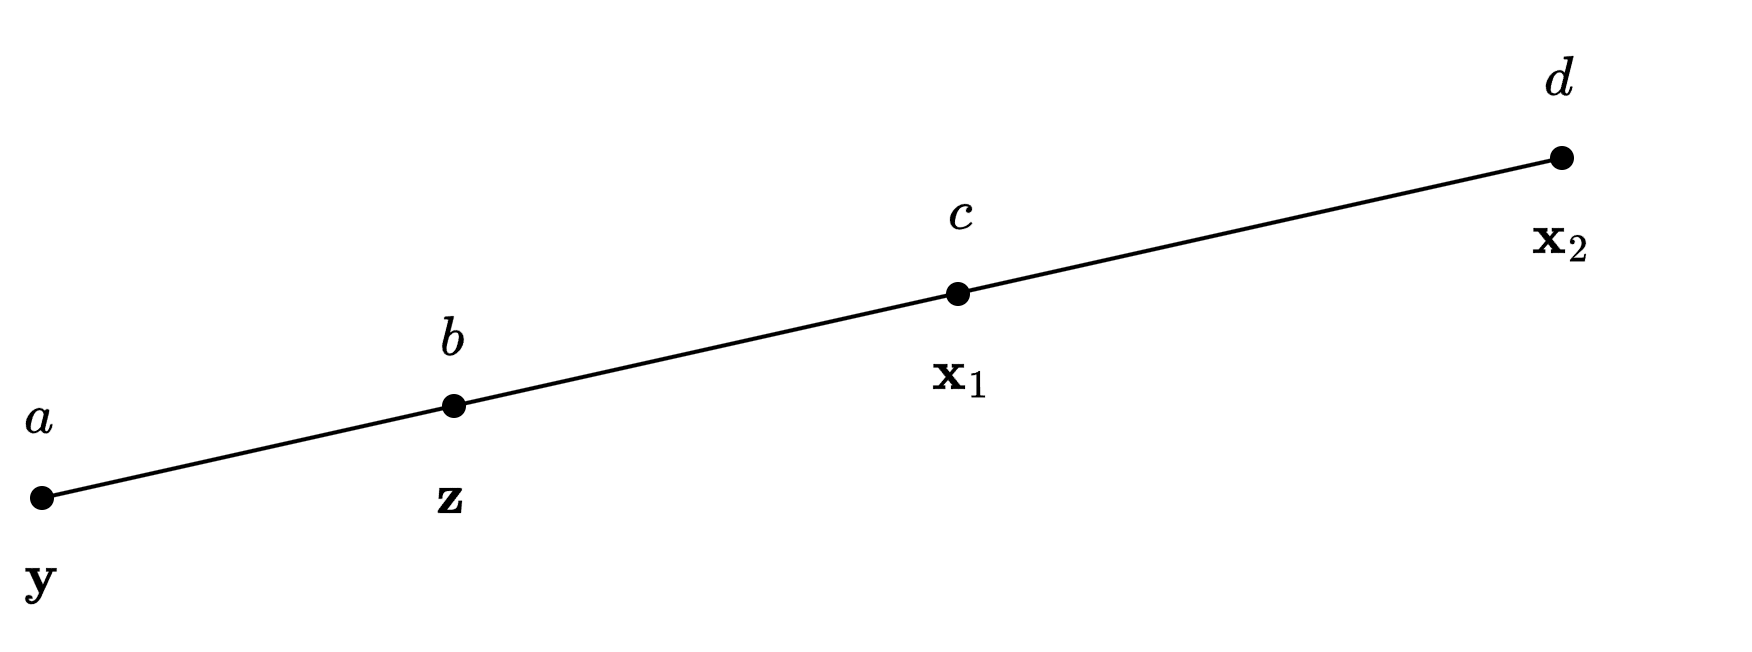
\includegraphics[width=0.25\linewidth]{images/line.png}
    \caption{Line with the point of previous problem}
\end{figure}
\begin{proof}  
    \begin{figure}[H]
        \centering
        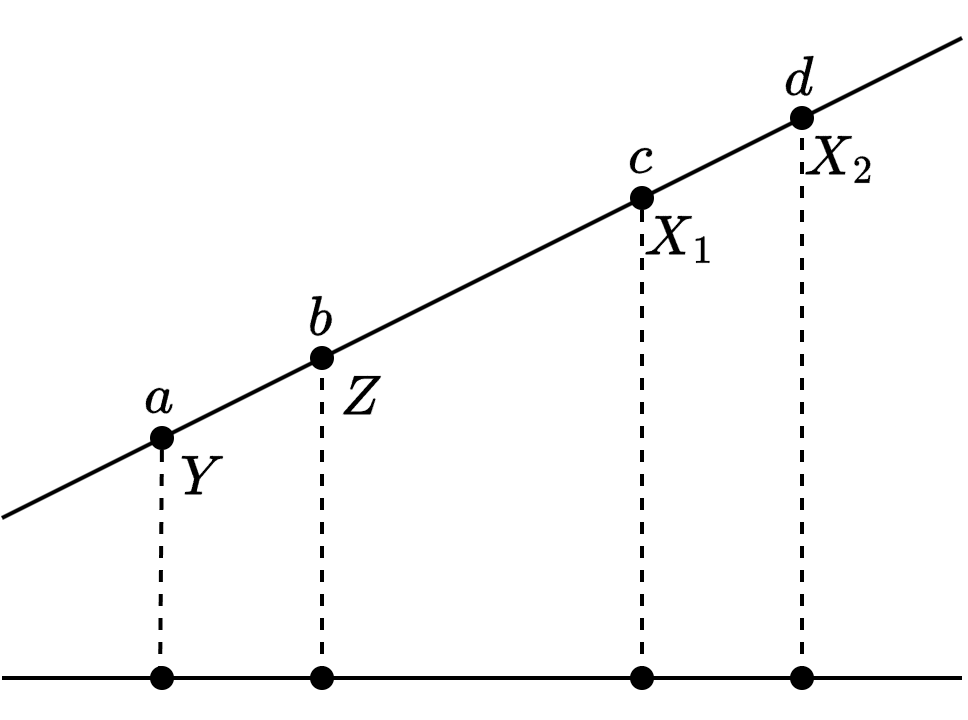
\includegraphics[width=0.3\linewidth]{images/abscissae.png}
    \end{figure}
    Since the abscissae are proportional, the abscissae can be replaced by the $x$-coordinate, as shown in the figure. 
    The relation:
    \[CR_{\mathbf{x}_1,\mathbf{x}_2,\mathbf{y},\mathbf{z}}=\dfrac{\left(\dfrac{c-a}{c-b}\right)}{\left(\dfrac{d-a}{d-b}\right)}\]
    still holds. 
    If we consider $\mathbf{y}={\begin{bmatrix} y & \ast & v \end{bmatrix}}^T$ and $\mathbf{z}={\begin{bmatrix} z & \ast & w \end{bmatrix}}^T$, we can determine that:
    \[\mathbf{x}_1=\begin{bmatrix} \alpha_1y+\beta_1z \\ \ast \\ \alpha_1v+\beta_1w \end{bmatrix} \qquad \mathbf{x}_2=\begin{bmatrix} \alpha_2y+\beta_2z \\ \ast \\ \alpha_2v+\beta_2w \end{bmatrix}\]
    The difference between the $x$ coordinates of $\mathbf{x}_1$ and $\mathbf{y}$ is:
    \[c-a=\dfrac{\beta_1(zv-yw)}{(\alpha_1y+\beta_1z)v}\]
    Similarly, the difference between the $x$ coordinates of $\mathbf{x}_1$ and $\mathbf{z}$ is:
    \[c-b=\dfrac{-\alpha_1(zv-yw)}{(\alpha_1y+\beta_1z)w}\]
    Substituting these expressions yields:
    \[\dfrac{c-a}{c-b}=-\dfrac{\beta_1w}{\alpha_1v} \qquad \dfrac{d-a}{d-b}=-\dfrac{\beta_2w}{\alpha_2v}\]
\end{proof}